\def\mytitle{ASSIGNMENT-3}
\def\myauthor{M Sai Santhosh Kumar}
\def\contact{santhoshmandarapu1221@gmail.com}
\def\mymodule{Future Wireless Communications (FWC)}
\documentclass[journal,12pt,twocolumn]{IEEEtran}
\usepackage{setspace}
\usepackage{gensymb}
\usepackage{xcolor}
\usepackage{caption}
\usepackage[hyphens,spaces,obeyspaces]{url}
\usepackage[cmex10]{amsmath}
\usepackage{mathtools}
\singlespacing
\usepackage{amsthm}
\usepackage{mathrsfs}
\usepackage{txfonts}
\usepackage{stfloats}
\usepackage{cite}
\usepackage{cases}
\usepackage{subfig}
\usepackage{longtable}
\usepackage{multirow}
\twocolumn
\usepackage{graphicx}
\graphicspath{{./images/}}
\usepackage[colorlinks,linkcolor={black},citecolor={blue!80!black},urlcolor={blue!80!black}]{hyperref}
\usepackage[parfill]{parskip}
\usepackage{lmodern}
\usepackage{tikz}
\usepackage{circuitikz}
\usepackage{karnaugh-map}
\usepackage{pgf}
\usepackage[hyphenbreaks]{breakurl}
\usepackage{tabularx}
\usetikzlibrary{calc}
\renewcommand*\familydefault{\sfdefault}
\usepackage{watermark}
\usepackage{lipsum}
\usepackage{xcolor}
\usepackage{listings}
\usepackage{float}
\usepackage{titlesec}
\DeclareMathOperator*{\Res}{Res}
%\renewcommand{\baselinestretch}{2}
\renewcommand\thesection{\arabic{section}}
\renewcommand\thesubsection{\thesection.\arabic{subsection}}
\renewcommand\thesubsubsection{\thesubsection.\arabic{subsubsection}}
\renewcommand\thesectiondis{\arabic{section}}
\renewcommand\thesubsectiondis{\thesectiondis.\arabic{subsection}}
\renewcommand\thesubsubsectiondis{\thesubsectiondis.\arabic{subsubsection}}
\hyphenation{op-tical net-works semi-conduc-tor}
\titlespacing{\subsection}{1pt}{\parskip}{3pt}
\titlespacing{\subsubsection}{0pt}{\parskip}{-\parskip}
\titlespacing{\paragraph}{0pt}{\parskip}{\parskip}
\newcommand{\figuremacro}[5]{
    \begin{figure}[#1]
        \centering
        \includegraphics[width=#5\columnwidth]{#2}
        \caption[#3]{\textbf{#3}#4}
        \label{fig:#2}
    \end{figure}
}
\lstset{
frame=single, 
breaklines=true,
columns=fullflexible
}
\title{\mytitle}
\author{\myauthor\hspace{1em}\\\contact\\IITH\hspace{0.5em}-\hspace{0.6em}\mymodule}
\date{23-03-2023}
\def\inputGnumericTable{}                           
\lstset{
frame=single, 
breaklines=true,
columns=fullflexible
}
\begin{document}
\theoremstyle{definition}
\newtheorem{theorem}{Theorem}[section]
\newtheorem{problem}{Problem}
\newtheorem{proposition}{Proposition}[section]
\newtheorem{lemma}{Lemma}[section]
\newtheorem{corollary}[theorem]{Corollary}
\newtheorem{example}{Example}[section]
\newtheorem{definition}{Definition}[section]
\newcommand{\BEQA}{\begin{eqnarray}}
\newcommand{\EEQA}{\end{eqnarray}}
\newcommand{\define}{\stackrel{\triangle}{=}}
\bibliographystyle{IEEEtran}
\vspace{3cm}
  \maketitle
  \tableofcontents
\section{Question}
        Consider the Boolean function z(a,b,c)
\begin{figure}[h]
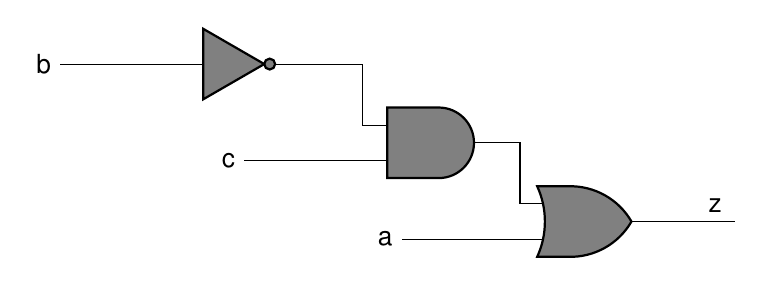
\begin{tikzpicture}
\ctikzset{
    logic ports=ieee,
    logic ports/scale=0.8,
    logic ports/fill=gray
}
 
\node[not port] (nota) at (0,0){};
\node[and port] (anda) at (2.5,-1){};
\node[or port]  (ora) at (4.5,-2){};
 
\draw (nota.out) -| (anda.in 1);
\draw (anda.out) -| (ora.in 1);
 
\draw (ora.out) -- ++(1,0) node[near end,above]{z};
 
\draw (nota.in 1) -- ++(-1.5,0)node[left]{b};
\draw (anda.in 2) -- ++(-1.5,0)node[left]{c};
\draw (ora.in 2) -- ++(-1.5,0)node[left] {a};
 
\end{tikzpicture}

\end{figure}
  Which of the following minterm lists represents the circuit given above?
\begin{enumerate}
\item $z=\sum(0,1,3,7)$
\item $z=\sum(1,4,5,6,7)$
\item $z=\sum(2,4,5,6,7)$
\item $z=\sum(2,3,5)$ 
\end{enumerate} 
\section{Components}
  \begin{tabularx}{0.4\textwidth} { 
  | >{\centering\arraybackslash}X 
  | >{\centering\arraybackslash}X 
  | >{\centering\arraybackslash}X
  | >{\centering\arraybackslash}X | }
\hline
 \textbf{Component}& \textbf{Values} & \textbf{Quantity}\\
\hline
Arduino & UNO & 1 \\  
\hline
JumperWires& M-M & 6 \\ 
\hline
Breadboard &  & 1 \\
\hline
LED & &1 \\
\hline
Resistor &220ohms & 1\\
\hline
\end{tabularx}
\begin{center}
Figure.a
\end{center}
\section{Truth Table}
  \begin{tabularx}{0.46\textwidth} { 
  | >{\centering\arraybackslash}X 
  | >{\centering\arraybackslash}X 
  | >{\centering\arraybackslash}X
  | >{\centering\arraybackslash}X 
  | >{\centering\arraybackslash}X 
  | >{\centering\arraybackslash}X 
  | >{\centering\arraybackslash}X 
  | >{\centering\arraybackslash}X 
  | >{\centering\arraybackslash}X 
  | >{\centering\arraybackslash}X | }
\hline
\textbf{a} & \textbf{b} & \textbf{c} & \textbf{z}\\
\hline
0 & 0 & 0 & 0  \\  
\hline
0 & 0 & 1 & 1  \\ 
\hline
0 & 1 & 0 & 0  \\
\hline
0 & 1 & 1 & 0  \\
\hline
1 & 0 & 0 & 1  \\  
\hline
1 & 0 & 1 & 1  \\ 
\hline
1 & 1 & 0 & 1  \\
\hline
1 & 1 & 1 & 1 \\
\hline
\end{tabularx}
\begin{center}
 Truth table Boolean Function "z"
\end{center}
\section{Logical Diagram}
\begin{figure}[h]
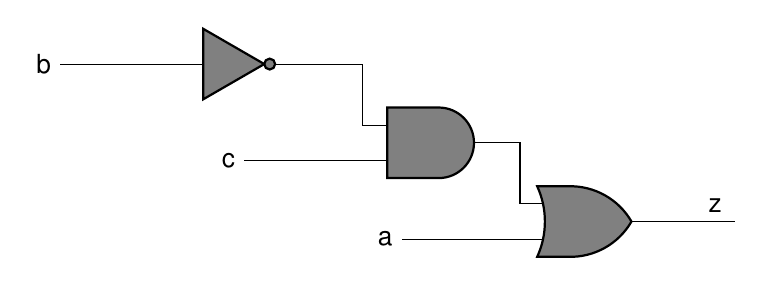
\begin{tikzpicture}
\ctikzset{
    logic ports=ieee,
    logic ports/scale=0.8,
    logic ports/fill=gray
}
 
\node[not port] (nota) at (0,0){};
\node[and port] (anda) at (2.5,-1){};
\node[or port]  (ora) at (4.5,-2){};
 
\draw (nota.out) -| (anda.in 1);
\draw (anda.out) -| (ora.in 1);
 
\draw (ora.out) -- ++(1,0) node[near end,above]{z};
 
\draw (nota.in 1) -- ++(-1.5,0)node[left]{b};
\draw (anda.in 2) -- ++(-1.5,0)node[left]{c};
\draw (ora.in 2) -- ++(-1.5,0)node[left] {a};
 
\end{tikzpicture}

\caption{Logical Diagram}
\label{fig:}
\end{figure}
\section{Implementation}
  \begin{tabularx}{0.46\textwidth} { 
  | >{\centering\arraybackslash}X 
  | >{\centering\arraybackslash}X 
  | >{\centering\arraybackslash}X  | }
\hline
\textbf{Arduino PIN} & \textbf{INPUT} & \textbf{OUTPUT} \\ 
\hline
\textbf 2 & a & \\
\hline
\textbf 3 & b & \\
\hline
\textbf 4 & c & \\
\hline
\textbf 5 & & z \\
\hline
\end{tabularx}
\begin{center}
    Connections
\end{center}
    \paragraph{$Procedure$}
    
    1. Connect the circuit as per the above table.\\
    2. Connnect the one end of the resistor to anode of LED and cathode of LED to ground.\\
    3. Connect the output pin to another end of resisor.\\
    4. Connect inputs to Vcc for logic 1, ground for logic 0.\\
    5. Execute the circuit using the below code.\\
   
\begin{tabularx}{0.46\textwidth} { 
  | >{\centering\arraybackslash}X |}
  \hline
  https://github.com/santhosh-1221/cs282020/blob/main/code/code.asm \\
  \hline
\end{tabularx}
   
6. Change the values of a,b,c in the code and verify the Truth Table.\\
\bibliographystyle{ieeetr}
\end{document}
